% Original pixels retain every icon, number and arrow; only explanatory labels are covered.
\begingroup
\begin{tikzpicture}[x=0.0112716763cm,y=-0.0112716763cm,
  every node/.style={inner sep=0pt,outer sep=0pt,align=center,font=\sffamily\fontsize{9.5}{11}\selectfont}]
  \node[anchor=north west] at (0,0) {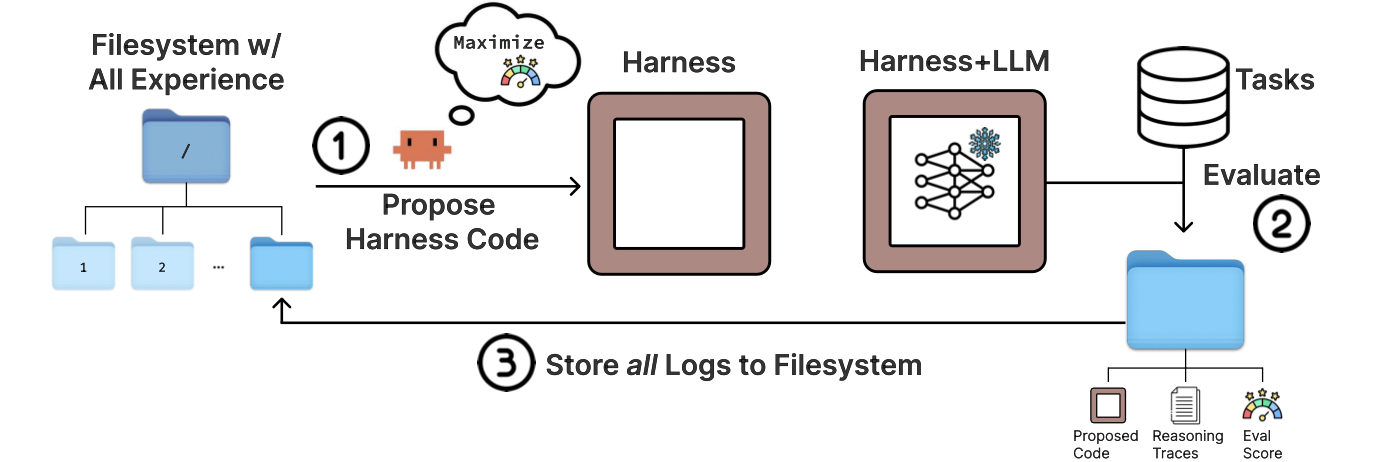
\includegraphics[width=15.6cm]{figures/metaharness.png}};
  \path[fill=white] (73,25) rectangle (313,99);
  \node[font=\sffamily\bfseries\fontsize{9.5}{11}\selectfont] at (194,62) {保存全部经验\\的文件系统};
  \path[fill=white] (450,29) rectangle (547,54);
  \node[font=\sffamily\bfseries\fontsize{7.5}{8.5}\selectfont] at (498,42) {最大化};
  \path[fill=white] (614,43) rectangle (775,80);
  \node[font=\sffamily\bfseries\fontsize{10}{11}\selectfont] at (683,62) {控制框架};
  \path[fill=white] (849,40) rectangle (1056,83);
  \node[font=\sffamily\bfseries\fontsize{9.5}{11}\selectfont] at (953,62) {控制框架＋LLM};
  \path[fill=white] (1232,60) rectangle (1332,96);
  \node[font=\sffamily\bfseries\fontsize{10}{11}\selectfont] at (1281,79) {任务};
  \path[fill=white] (336,192) rectangle (582,258);
  \node[font=\sffamily\bfseries\fontsize{9.5}{11}\selectfont] at (462,224) {提出\\控制框架代码};
  \path[fill=white] (1197,157) rectangle (1353,192);
  \node[font=\sffamily\bfseries\fontsize{10}{11}\selectfont] at (1272,176) {评估};
  \path[fill=white] (543,347) rectangle (1030,387);
  \node[font=\sffamily\bfseries\fontsize{9.5}{11}\selectfont] at (785,368) {将全部日志存入文件系统};
  \path[fill=white] (1065,428) rectangle (1147,462);
  \path[fill=white] (1149,428) rectangle (1228,462);
  \path[fill=white] (1237,428) rectangle (1307,462);
  \node[font=\sffamily\fontsize{7.5}{8}\selectfont] at (1107,463) {提出的\\代码};
  \node[font=\sffamily\fontsize{7.5}{8}\selectfont] at (1188,463) {推理\\轨迹};
  \node[font=\sffamily\fontsize{7.5}{8}\selectfont] at (1271,463) {评估\\得分};
\end{tikzpicture}
\endgroup
